% This is part of the Jabuti 1.0 Manual.
% Copyright 2003 (c) Auri Marcelo Rizzo Vicenzi, Marcio Eduardo Delamaro,
% Jose Carlos Maldonado.
% See the file FDL.TXT for copying conditions.

\begin{figure}[!ht]
\begin{center}
\subfigure[]{\label{fig:initial-summary-class-pri-nodes}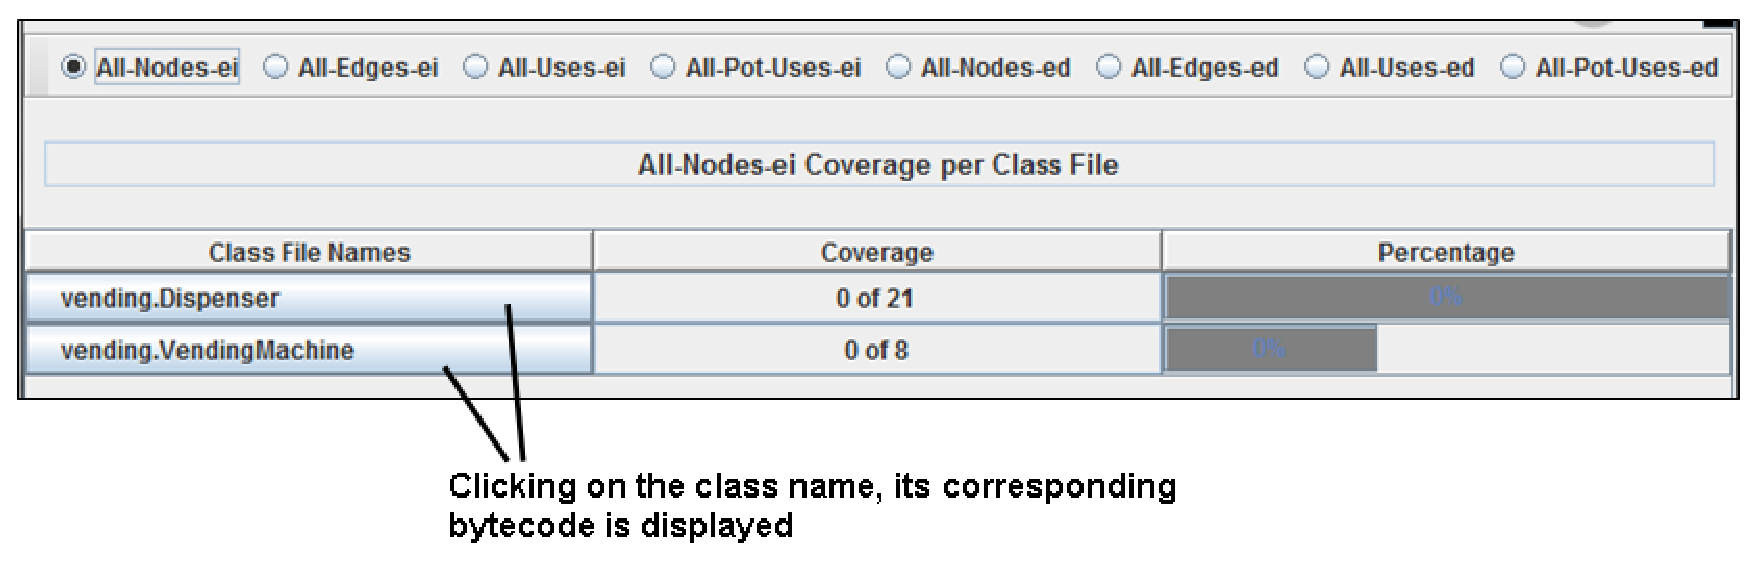
\includegraphics[width=0.70\textwidth]{fig/summary-by-class-pri-nodes-edited.eps}}

\subfigure[]{\label{fig:initial-summary-class-pri-edges}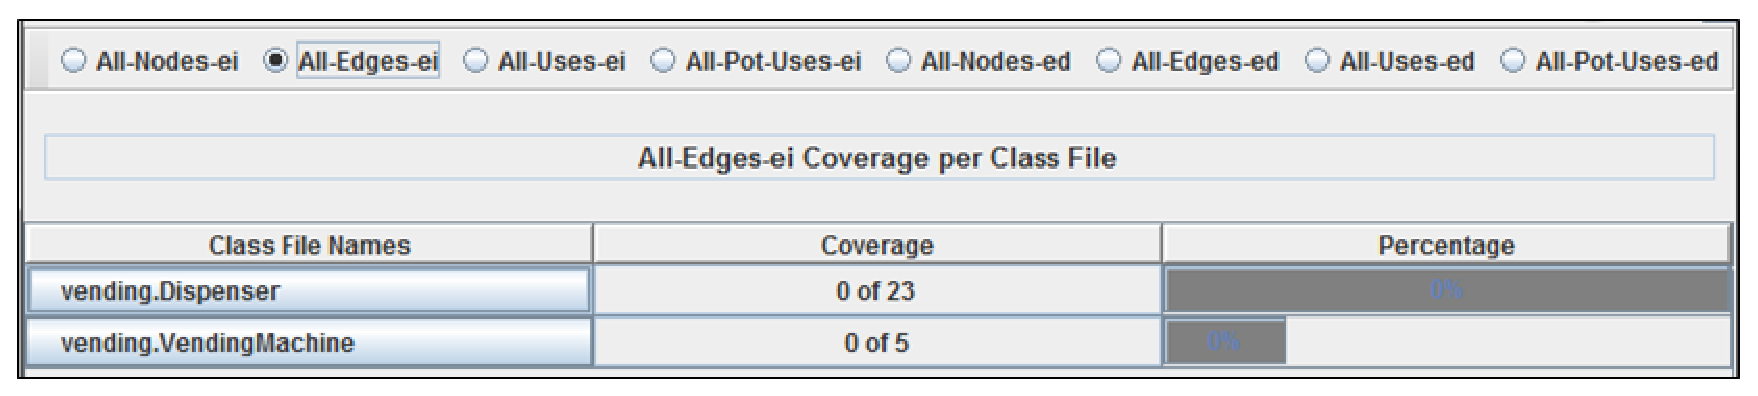
\includegraphics[width=0.70\textwidth]{fig/summary-by-class-pri-edges-edited.eps}}

\subfigure[]{\label{fig:initial-summary-class-pri-uses}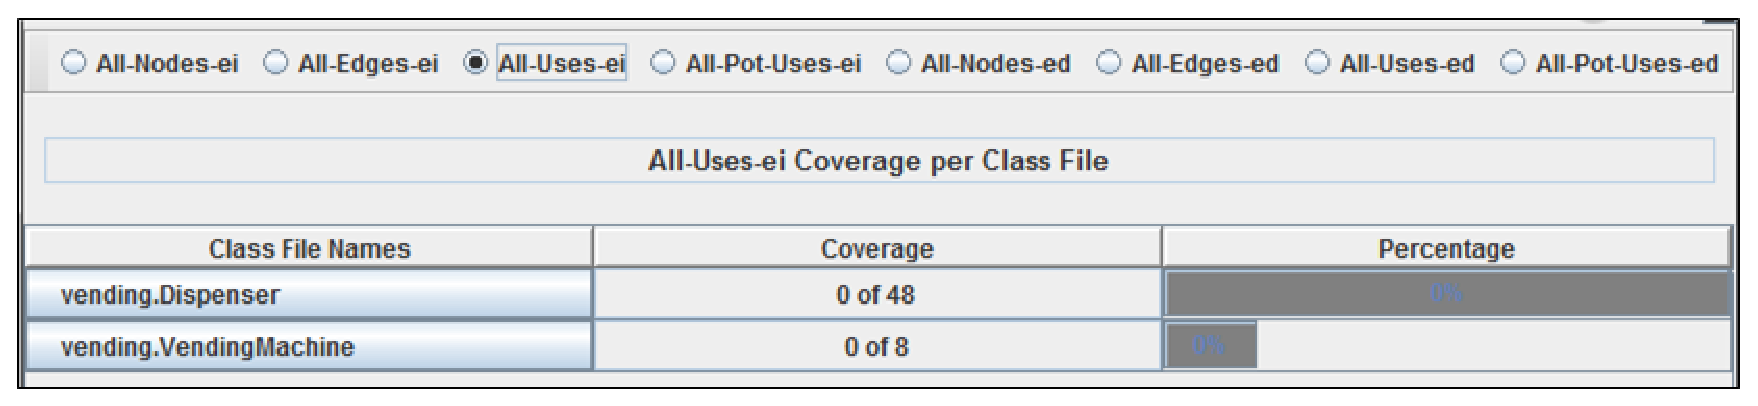
\includegraphics[width=0.70\textwidth]{fig/summary-by-class-pri-uses-edited.eps}}

\caption{Initial summary per class file: (a) \pk{All-Pri-Nodes}
criterion, (b) \pk{All-Pri-Edges} criterion, and (c)
\pk{All-Pri-Uses} criterion.}\label{fig:initial-summary-class}
\end{center}
\end{figure}
